\section{Результаты опробования программ}
\label{sec:Results_8} \index{Results_8}
\large 

\subsection{Основные результаты}
Получена приблизительная сложность работы усовершенствованного алгоритма. В случае случайного графа, модернизация алгоритма дает неплохой результат на небольших размерах. Но эффективность стремительно падает, при увеличении количества вершин графа.

Время работы программы в зависимости от размера графа на среднем по мощности компьютере (затраты оперативной памяти $\thickapprox 2\times 10^9$ байт):
\begin{enumerate}
\item  До 200 вершин - $<$ 1 секунды.
\item  В пределах 300 вершин - около 2 секунд.
\item  400 — 500 вершин - до 20 секунд.
\end{enumerate}




Приблизительная оценка времени работы программы на мощной вычислительной технике:
оперативная память $10^{14}$ байт,
количество операций в секунду $10^{15}$ [5].
\begin{enumerate}
\item 1000 вершин - $<$ 1 секунды  ($10^{12}$  операций).
\item 3000 вершин - $<$ 5 секунд ($5\times 10^{15}$ операций).
\item 10000 вершин - около $2,5$ часов ($10^{19}$ операций).
\item 100000 вершин - около 320000 лет ($10 ^{28}$ операций).
\end{enumerate}
В последнем случае требуется $10^{21}$ байт оперативной памяти.


\subsection{Масштабируемость реализации алгоритма}
Исследование проводилось на суперкомпьютере "Ломоносов" \cite{Voevodin_article_1}

Набор и границы значений изменяемых параметров запуска реализации алгоритма: 

\begin{enumerate}
\item число процессоров [4 : 128] с шагом $ 2^n$ (точки отображены с шагом 4, с усреднением результата на промежуточных точках);
\item Размер матрицы [300 : 1000].
\end{enumerate}

В результате проведённых экспериментов был получен следующий диапазон алгоритма:

\begin{itemize}
\item минимальная эффективность реализации 17,44%;
\item максимальная эффективность реализации 88,73%.
\end{itemize}

На следующих изображениях приведены графики производительности и эффективности выбранной реализации поиска автоморфизмов графов в зависимости от изменяемых параметров запуска.

\begin{figure}[ht]
\centering 
    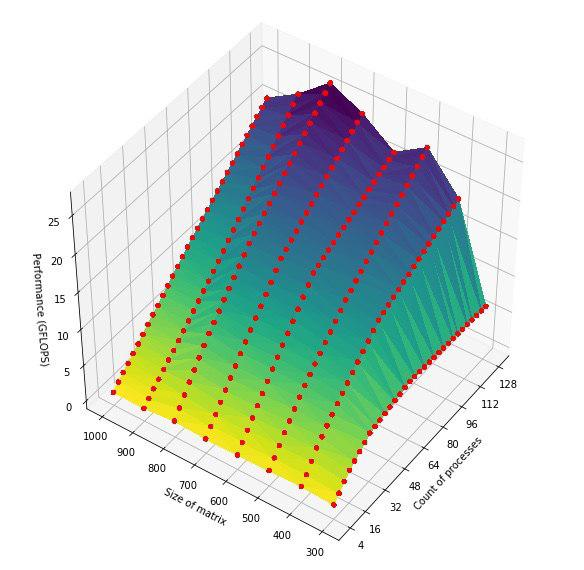
\includegraphics[scale=0.8]{image/p.jpg}
    \caption{Параллельная реализация алгоритма поиска автоморфизмов. Изменение производительности в зависимости от числа процессоров и размера матрицы.}
    \label{srg}
\end{figure}

\begin{figure}[ht]
\centering 
    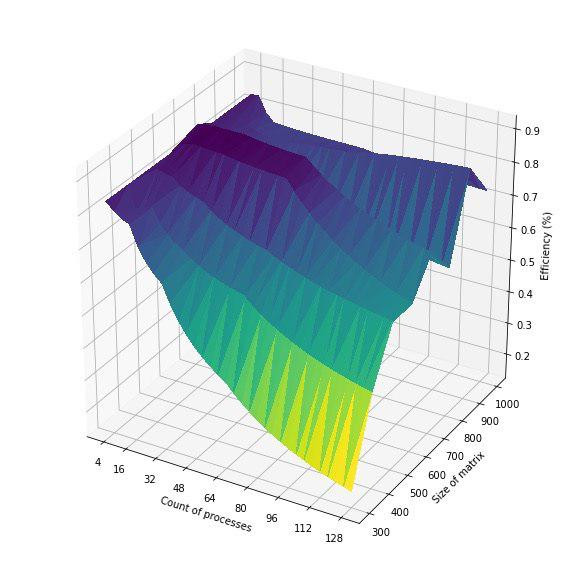
\includegraphics[scale=0.8]{image/ef.jpg}
    \caption{Параллельная реализация алгоритма поиска автоморфизмов. Изменение эффективности в зависимости от числа процессоров и размера матрицы.}
    \label{srg}
\end{figure}

Оценки масштабируемости выбранной реализации:
\begin{itemize}
\item По числу процессов: -0,00837.
\item По размеру задачи: 0,04612. 
\item По двум направлениям: 0,00253.
\end{itemize}
